% Options for packages loaded elsewhere
\PassOptionsToPackage{unicode}{hyperref}
\PassOptionsToPackage{hyphens}{url}
%
\documentclass[
]{article}
\usepackage{amsmath,amssymb}
\usepackage{lmodern}
\usepackage{iftex}
\ifPDFTeX
  \usepackage[T1]{fontenc}
  \usepackage[utf8]{inputenc}
  \usepackage{textcomp} % provide euro and other symbols
\else % if luatex or xetex
  \usepackage{unicode-math}
  \defaultfontfeatures{Scale=MatchLowercase}
  \defaultfontfeatures[\rmfamily]{Ligatures=TeX,Scale=1}
\fi
% Use upquote if available, for straight quotes in verbatim environments
\IfFileExists{upquote.sty}{\usepackage{upquote}}{}
\IfFileExists{microtype.sty}{% use microtype if available
  \usepackage[]{microtype}
  \UseMicrotypeSet[protrusion]{basicmath} % disable protrusion for tt fonts
}{}
\makeatletter
\@ifundefined{KOMAClassName}{% if non-KOMA class
  \IfFileExists{parskip.sty}{%
    \usepackage{parskip}
  }{% else
    \setlength{\parindent}{0pt}
    \setlength{\parskip}{6pt plus 2pt minus 1pt}}
}{% if KOMA class
  \KOMAoptions{parskip=half}}
\makeatother
\usepackage{xcolor}
\usepackage[margin=1in]{geometry}
\usepackage{color}
\usepackage{fancyvrb}
\newcommand{\VerbBar}{|}
\newcommand{\VERB}{\Verb[commandchars=\\\{\}]}
\DefineVerbatimEnvironment{Highlighting}{Verbatim}{commandchars=\\\{\}}
% Add ',fontsize=\small' for more characters per line
\usepackage{framed}
\definecolor{shadecolor}{RGB}{248,248,248}
\newenvironment{Shaded}{\begin{snugshade}}{\end{snugshade}}
\newcommand{\AlertTok}[1]{\textcolor[rgb]{0.94,0.16,0.16}{#1}}
\newcommand{\AnnotationTok}[1]{\textcolor[rgb]{0.56,0.35,0.01}{\textbf{\textit{#1}}}}
\newcommand{\AttributeTok}[1]{\textcolor[rgb]{0.77,0.63,0.00}{#1}}
\newcommand{\BaseNTok}[1]{\textcolor[rgb]{0.00,0.00,0.81}{#1}}
\newcommand{\BuiltInTok}[1]{#1}
\newcommand{\CharTok}[1]{\textcolor[rgb]{0.31,0.60,0.02}{#1}}
\newcommand{\CommentTok}[1]{\textcolor[rgb]{0.56,0.35,0.01}{\textit{#1}}}
\newcommand{\CommentVarTok}[1]{\textcolor[rgb]{0.56,0.35,0.01}{\textbf{\textit{#1}}}}
\newcommand{\ConstantTok}[1]{\textcolor[rgb]{0.00,0.00,0.00}{#1}}
\newcommand{\ControlFlowTok}[1]{\textcolor[rgb]{0.13,0.29,0.53}{\textbf{#1}}}
\newcommand{\DataTypeTok}[1]{\textcolor[rgb]{0.13,0.29,0.53}{#1}}
\newcommand{\DecValTok}[1]{\textcolor[rgb]{0.00,0.00,0.81}{#1}}
\newcommand{\DocumentationTok}[1]{\textcolor[rgb]{0.56,0.35,0.01}{\textbf{\textit{#1}}}}
\newcommand{\ErrorTok}[1]{\textcolor[rgb]{0.64,0.00,0.00}{\textbf{#1}}}
\newcommand{\ExtensionTok}[1]{#1}
\newcommand{\FloatTok}[1]{\textcolor[rgb]{0.00,0.00,0.81}{#1}}
\newcommand{\FunctionTok}[1]{\textcolor[rgb]{0.00,0.00,0.00}{#1}}
\newcommand{\ImportTok}[1]{#1}
\newcommand{\InformationTok}[1]{\textcolor[rgb]{0.56,0.35,0.01}{\textbf{\textit{#1}}}}
\newcommand{\KeywordTok}[1]{\textcolor[rgb]{0.13,0.29,0.53}{\textbf{#1}}}
\newcommand{\NormalTok}[1]{#1}
\newcommand{\OperatorTok}[1]{\textcolor[rgb]{0.81,0.36,0.00}{\textbf{#1}}}
\newcommand{\OtherTok}[1]{\textcolor[rgb]{0.56,0.35,0.01}{#1}}
\newcommand{\PreprocessorTok}[1]{\textcolor[rgb]{0.56,0.35,0.01}{\textit{#1}}}
\newcommand{\RegionMarkerTok}[1]{#1}
\newcommand{\SpecialCharTok}[1]{\textcolor[rgb]{0.00,0.00,0.00}{#1}}
\newcommand{\SpecialStringTok}[1]{\textcolor[rgb]{0.31,0.60,0.02}{#1}}
\newcommand{\StringTok}[1]{\textcolor[rgb]{0.31,0.60,0.02}{#1}}
\newcommand{\VariableTok}[1]{\textcolor[rgb]{0.00,0.00,0.00}{#1}}
\newcommand{\VerbatimStringTok}[1]{\textcolor[rgb]{0.31,0.60,0.02}{#1}}
\newcommand{\WarningTok}[1]{\textcolor[rgb]{0.56,0.35,0.01}{\textbf{\textit{#1}}}}
\usepackage{graphicx}
\makeatletter
\def\maxwidth{\ifdim\Gin@nat@width>\linewidth\linewidth\else\Gin@nat@width\fi}
\def\maxheight{\ifdim\Gin@nat@height>\textheight\textheight\else\Gin@nat@height\fi}
\makeatother
% Scale images if necessary, so that they will not overflow the page
% margins by default, and it is still possible to overwrite the defaults
% using explicit options in \includegraphics[width, height, ...]{}
\setkeys{Gin}{width=\maxwidth,height=\maxheight,keepaspectratio}
% Set default figure placement to htbp
\makeatletter
\def\fps@figure{htbp}
\makeatother
\setlength{\emergencystretch}{3em} % prevent overfull lines
\providecommand{\tightlist}{%
  \setlength{\itemsep}{0pt}\setlength{\parskip}{0pt}}
\setcounter{secnumdepth}{-\maxdimen} % remove section numbering
\ifLuaTeX
  \usepackage{selnolig}  % disable illegal ligatures
\fi
\IfFileExists{bookmark.sty}{\usepackage{bookmark}}{\usepackage{hyperref}}
\IfFileExists{xurl.sty}{\usepackage{xurl}}{} % add URL line breaks if available
\urlstyle{same} % disable monospaced font for URLs
\hypersetup{
  pdftitle={Models},
  hidelinks,
  pdfcreator={LaTeX via pandoc}}

\title{Models}
\author{}
\date{\vspace{-2.5em}2023-03-14}

\begin{document}
\maketitle

The main functions of the \texttt{StormR} package, i.e., the
\texttt{SpatialBehaviour()} and \texttt{TemporalBehaviour()} functions,
allow to compute summary statistics from wind speed and direction field
computed using storm track data. Wind fields can be computed using
different sets of parametric models. Three models described by Holland
(1980), Willoughby et al.~(2006), and Boose et al.~(2004) are
implemented in this package. Those models compute radial wind speed
\(v_r\) (in \(m.s^{-1}\)) at the distance \(r\) (in \(km\)) from the
centre of the storm. In both the \texttt{SpatialBehaviour()} and
\texttt{TemporalBehaviour()} functions the model can be defined using
the \texttt{method} argument.

The original Holland (1980) and Willoughby et al.~(2006) models are
symmetrical, however winds are rarely symmetric around the centre of a
storm, notably because of the translation movement of the storm. It is
therefore more realistic to add asymmetry to the wind field generated by
these models (Yan and Zhang, 2022). We implemented two formula to add
asymmetry to Holland (1980) and Willoughby et al.~(2006) models. These
formula have been developed by Miyazaki et al.~(1962) and Chen (1994)
and can be used using the \texttt{asymmetry} argument of the
\texttt{SpatialBehaviour()} and \texttt{TemporalBehaviour()} functions.

The third model developed by Boose et al.~(2004) is an asymmetrical
version of the Holland (1980) model. Contrary to the Holland (1980) and
Willoughby et al.~(2006), this model has different parameter settings on
water and lands. Below we describe the models and compared wind speed
profiles generated by the different sets of models using the
\texttt{SpatialBehaviour()} function and the \texttt{product="Profiles}
argument. In these examples we use the track data for the tropical
cyclone Pam (2015) provided in the \texttt{test\_dataset} dataset of the
package.

\begin{Shaded}
\begin{Highlighting}[]
\NormalTok{st }\OtherTok{\textless{}{-}} \FunctionTok{Storms}\NormalTok{(}\AttributeTok{loi =} \StringTok{"Vanuatu"}\NormalTok{, }\AttributeTok{names =} \StringTok{"PAM"}\NormalTok{,}\AttributeTok{verbose=}\DecValTok{0}\NormalTok{)}
\end{Highlighting}
\end{Shaded}

\hypertarget{holland-1980-symmetric-wind-field}{%
\subsubsection{Holland (1980) symmetric wind
field}\label{holland-1980-symmetric-wind-field}}

The Holland (1980) model is a simple model that only require few basic
parameters and has a wide applicability.

\[
v_r = \sqrt{\frac{b}{\rho} \times \left(\frac{R_m}{r}\right)^b \times (p_{oci} - p_c) \times e^{-\left(\frac{R_m}{r}\right)^b} + \left(\frac{r \times f}{2}\right)^2} - \left(\frac{r \times f}{2}\right)
\] where, \(v_r\) is the radial wind speed (in \(m.s^{-1}\)) \(r\) is
the distance to the eye of the storm (in \(km\)) \(R_m\) is the radius
of maximum sustained wind speed (in \(km\)) \(p_c\) is the pressure at
the centre of the storm (in \(mb\)) \(p_{oci}\) is the pressure at
outermost closed isobar of the storm (in \(mb\)) \(\rho\) is the air
density set to \(1.15 kg.m^{-3}\)
\(f = 2 \times 7.29 \times 10^{-5} \sin(\phi)\) is the Coriolis force
(in \(N.kg^{-1}\), with \(\phi\) being the latitude)
\(b = \frac{\rho \times e \times v_m^2}{p_{oci} - p_c}\) is the shape
parameter, with \(e\) being the base of natural logarithms
\textasciitilde2.718282 and \(v_m\) the maximum sustained wind speed (in
\(m.s^{-1}\))

\hypertarget{willoughby-et-al.-2006-symmetric-wind-field}{%
\subsubsection{Willoughby et al.~(2006) symmetric wind
field}\label{willoughby-et-al.-2006-symmetric-wind-field}}

The Willoughby et al.~(2006) model is a two sections model in which wind
increase as a power of radius inside the eye and decay exponentially
outside the eye after a smooth polynomial transition across the eye wall
(see also Willoughby 1995, Willoughby et al.~2004).

\[
\left\{
\begin{aligned}
v_r &= v_m \times \left(\frac{r}{R_m}\right)^{n} \quad if \quad r < R_m \\
v_r &= v_m \times \left((1-A) \times e^{-\frac{|r-R_m|}{X1}} + A \times e^{-\frac{|r-R_m|}{X2}}\right) \quad if \quad r \geq R_m \\
\end{aligned}
\right.
\] where, \(v_r\) is the radial wind speed (in \(m.s^{-1}\)) \(r\) is
the distance to the eye of the storm (in \(km\)) \(v_m\) is the maximum
sustained wind speed (in \(m.s^{-1}\)) \(R_m\) is the radius of maximum
sustained wind speed (in \(km\))
\(X1 = 287.6 - 1.942 \times v_m + 7.799 \times \ln(R_m) + 1.819 \times |\phi|\)
\(X2 = 25\)
\(n = 2.1340 + 0.0077 \times v_m - 0.4522 \times \ln(R_m) - 0.0038 \times |\phi|\)
\(A = 0.5913 + 0.0029 \times v_m - 0.1361 \times \ln(R_m) - 0.0042 \times |\phi|\)
and \(A\ge0\) \(\phi\) is the latitude of the center of the storm

\hypertarget{adding-asymmetry-to-holland-1980-and-willoughby-et-al.-2006-wind-fields}{%
\subsubsection{Adding asymmetry to Holland (1980) and Willoughby et
al.~(2006) wind
fields}\label{adding-asymmetry-to-holland-1980-and-willoughby-et-al.-2006-wind-fields}}

The asymmetry generated by the translation speed of the storm can be
added as follows:

\(\vec{V} = \vec{V_c} + C \times \vec{V_t}\)

where, \(\vec{V}\) is the combined, asymmetric wind field \(\vec{V_c}\)
is symmetric wind field \(\vec{V_t}\) is the translation speed of the
storm \(C\) is function of \(r\), the distance to the eye of the storm
(in \(km\))

\hypertarget{miyazaki-et-al.-1962}{%
\paragraph{Miyazaki et al.~1962}\label{miyazaki-et-al.-1962}}

\(C = e^{(-\frac{r}{500} \times \pi)}\)

\hypertarget{chen-1994}{%
\paragraph{Chen 1994}\label{chen-1994}}

\(C = \frac{3 \times R_m^{\frac{3}{2}} \times r^{\frac{3}{2}}}{R_m^3 + r^3 +R_m^{\frac{3}{2}} \times r^{\frac{3}{2}}}\)

where, \(R_m\) is the radius of maximum sustained wind speed (in \(km\))

\hypertarget{boose-et-al.-2004-asymmertric-model}{%
\subsubsection{Boose et al.~(2004) asymmertric
model}\label{boose-et-al.-2004-asymmertric-model}}

The Boose et al.~(2004) model or ``HURRECON'' model is a modification of
the Holland (1980) model (see also Boose et al.~2001). In addition to
adding asymmetry this model also include a different parametrisation on
lands and waters.

\[
v_r = F\left(v_m - S \times (1 - \sin(T)) \times \frac{v_h}{2} \right) \times \sqrt{\left(\frac{R_m}{r}\right)^b \times e^{1 - \left(\frac{R_m}{r}\right)^b}}
\]

\(v_r\) is the radial wind speed (in \(m.s^{-1}\)) \(v_h\) is the storm
velocity (in \(m.s^{-1}\)) \(r\) is the distance to the eye of the storm
(in \(km\)) \(v_m\) is the maximum sustained wind speed (in
\(m.s^{-1}\)) \(R_m\) is the radius of maximum sustained wind speed (in
\(km\)) \(p_c\) is the pressure at the centre of the storm (\(pressure\)
in \(mb\)) \(p_{oci}\) is the pressure at outermost closed isobar of the
storm (in \(mb\)) \(\rho = 1.15\) is the air density (in \(kg.m^{-3}\))
\(b = \frac{\rho \times e \times v_m^2}{p_{oci} - p_c}\) is the shape
parameter \(F\) is a scaling parameter for friction (\(1.0\) in water,
\(0.8\) in land) \(S\) is a scaling parameter for asymmetry (\(1.0\))
\(T\) oriented angle (clockwise/counter clockwise in Northern/Southern
Hemisphere) between forward trajectory of the storm and a radial line
from the eye of the storm to point \(r\) \(S\) Asymmetry coefficient
(usually set to 1)

if \(R_m\) is not provided then it is approximated using an empirical
formula derived from Willoughby et al.~(2006)
\(R_m = 46.4e^{(-0.0155 \times v_m + 0.0169 \times |\phi|)}\)

\begin{Shaded}
\begin{Highlighting}[]
\NormalTok{st }\OtherTok{\textless{}{-}} \FunctionTok{Storms}\NormalTok{(}\AttributeTok{loi =} \FunctionTok{c}\NormalTok{(}\FloatTok{168.33}\NormalTok{,}\SpecialCharTok{{-}}\FloatTok{17.73}\NormalTok{), }\AttributeTok{names =} \StringTok{"PAM"}\NormalTok{,}\AttributeTok{verbose=}\DecValTok{0}\NormalTok{)}
\NormalTok{PAM}\OtherTok{\textless{}{-}}\FunctionTok{getObs}\NormalTok{(st,}\AttributeTok{name=}\StringTok{"PAM"}\NormalTok{)}
\FunctionTok{par}\NormalTok{(}\AttributeTok{mfrow=}\FunctionTok{c}\NormalTok{(}\DecValTok{1}\NormalTok{,}\DecValTok{2}\NormalTok{))}
\NormalTok{pf }\OtherTok{\textless{}{-}} \FunctionTok{spatialBehaviour}\NormalTok{(st,}\AttributeTok{product=}\StringTok{"Profiles"}\NormalTok{,}\AttributeTok{method=}\StringTok{"Holland"}\NormalTok{,}\AttributeTok{asymmetry=}\StringTok{"None"}\NormalTok{,}\AttributeTok{verbose=}\DecValTok{0}\NormalTok{)}
\NormalTok{terra}\SpecialCharTok{::}\FunctionTok{plot}\NormalTok{(pf}\SpecialCharTok{$}\NormalTok{PAM\_Speed\_41,}\AttributeTok{main=}\StringTok{"Holland (1980)"}\NormalTok{,}\AttributeTok{cex.main=}\FloatTok{0.8}\NormalTok{)}
\NormalTok{terra}\SpecialCharTok{::}\FunctionTok{plot}\NormalTok{(countriesHigh,}\AttributeTok{add=}\ConstantTok{TRUE}\NormalTok{)}
\FunctionTok{lines}\NormalTok{(PAM}\SpecialCharTok{$}\NormalTok{lon,PAM}\SpecialCharTok{$}\NormalTok{lat,}\AttributeTok{lty=}\DecValTok{3}\NormalTok{)}
\NormalTok{pf }\OtherTok{\textless{}{-}} \FunctionTok{spatialBehaviour}\NormalTok{(st,}\AttributeTok{product=}\StringTok{"Profiles"}\NormalTok{,}\AttributeTok{method=}\StringTok{"Willoughby"}\NormalTok{,}\AttributeTok{asymmetry=}\StringTok{"None"}\NormalTok{,}\AttributeTok{verbose=}\DecValTok{0}\NormalTok{)}
\NormalTok{terra}\SpecialCharTok{::}\FunctionTok{plot}\NormalTok{(pf}\SpecialCharTok{$}\NormalTok{PAM\_Speed\_41,}\AttributeTok{main=}\StringTok{"Willoughby et al. (2006)"}\NormalTok{,}\AttributeTok{cex.main=}\FloatTok{0.8}\NormalTok{)}
\NormalTok{terra}\SpecialCharTok{::}\FunctionTok{plot}\NormalTok{(countriesHigh,}\AttributeTok{add=}\ConstantTok{TRUE}\NormalTok{)}
\FunctionTok{lines}\NormalTok{(PAM}\SpecialCharTok{$}\NormalTok{lon,PAM}\SpecialCharTok{$}\NormalTok{lat,}\AttributeTok{lty=}\DecValTok{3}\NormalTok{)}
\end{Highlighting}
\end{Shaded}

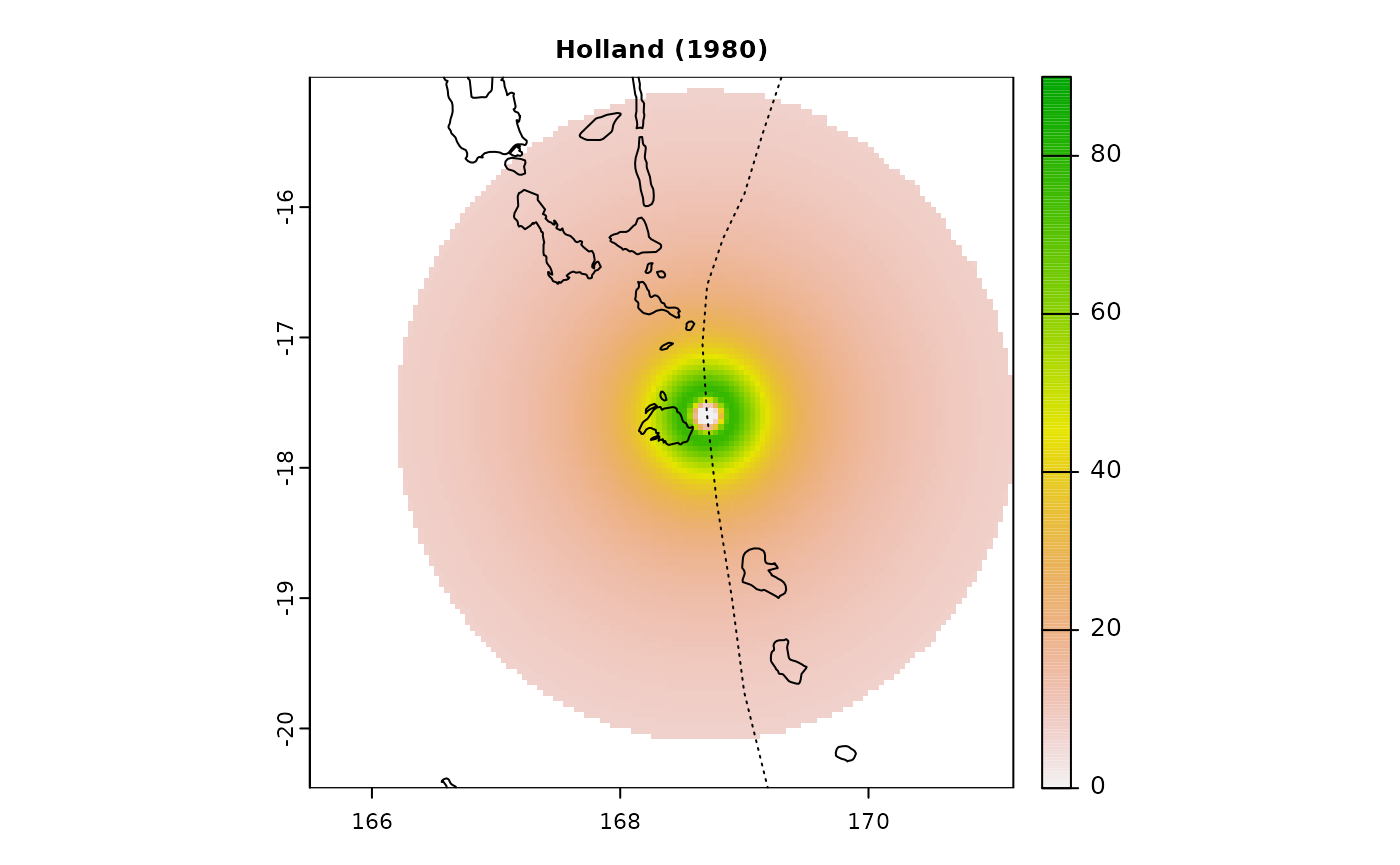
\includegraphics{Models_files/figure-latex/unnamed-chunk-2-1.pdf}

\begin{Shaded}
\begin{Highlighting}[]
\FunctionTok{par}\NormalTok{(}\AttributeTok{mfrow=}\FunctionTok{c}\NormalTok{(}\DecValTok{1}\NormalTok{,}\DecValTok{2}\NormalTok{))}
\NormalTok{pf }\OtherTok{\textless{}{-}} \FunctionTok{spatialBehaviour}\NormalTok{(st,}\AttributeTok{product=}\StringTok{"Profiles"}\NormalTok{,}\AttributeTok{method=}\StringTok{"Holland"}\NormalTok{,}\AttributeTok{asymmetry=}\StringTok{"Miyazaki"}\NormalTok{,}\AttributeTok{verbose=}\DecValTok{0}\NormalTok{)}
\NormalTok{terra}\SpecialCharTok{::}\FunctionTok{plot}\NormalTok{(pf}\SpecialCharTok{$}\NormalTok{PAM\_Speed\_41,}\AttributeTok{main=}\StringTok{"Holland (1980) + Miyazaki et al. (1962)"}\NormalTok{,}\AttributeTok{cex.main=}\FloatTok{0.8}\NormalTok{)}
\NormalTok{terra}\SpecialCharTok{::}\FunctionTok{plot}\NormalTok{(countriesHigh,}\AttributeTok{add=}\ConstantTok{TRUE}\NormalTok{)}
\FunctionTok{lines}\NormalTok{(PAM}\SpecialCharTok{$}\NormalTok{lon,PAM}\SpecialCharTok{$}\NormalTok{lat,}\AttributeTok{lty=}\DecValTok{3}\NormalTok{)}
\NormalTok{pf }\OtherTok{\textless{}{-}} \FunctionTok{spatialBehaviour}\NormalTok{(st,}\AttributeTok{product=}\StringTok{"Profiles"}\NormalTok{,}\AttributeTok{method=}\StringTok{"Willoughby"}\NormalTok{,}\AttributeTok{asymmetry=}\StringTok{"Miyazaki"}\NormalTok{,}\AttributeTok{verbose=}\DecValTok{0}\NormalTok{)}
\NormalTok{terra}\SpecialCharTok{::}\FunctionTok{plot}\NormalTok{(pf}\SpecialCharTok{$}\NormalTok{PAM\_Speed\_41,}\AttributeTok{main=}\StringTok{"Willoughby et al. (2006) + Miyazaki et al. (1962)"}\NormalTok{,}\AttributeTok{cex.main=}\FloatTok{0.8}\NormalTok{)}
\NormalTok{terra}\SpecialCharTok{::}\FunctionTok{plot}\NormalTok{(countriesHigh,}\AttributeTok{add=}\ConstantTok{TRUE}\NormalTok{)}
\FunctionTok{lines}\NormalTok{(PAM}\SpecialCharTok{$}\NormalTok{lon,PAM}\SpecialCharTok{$}\NormalTok{lat,}\AttributeTok{lty=}\DecValTok{3}\NormalTok{)}
\end{Highlighting}
\end{Shaded}

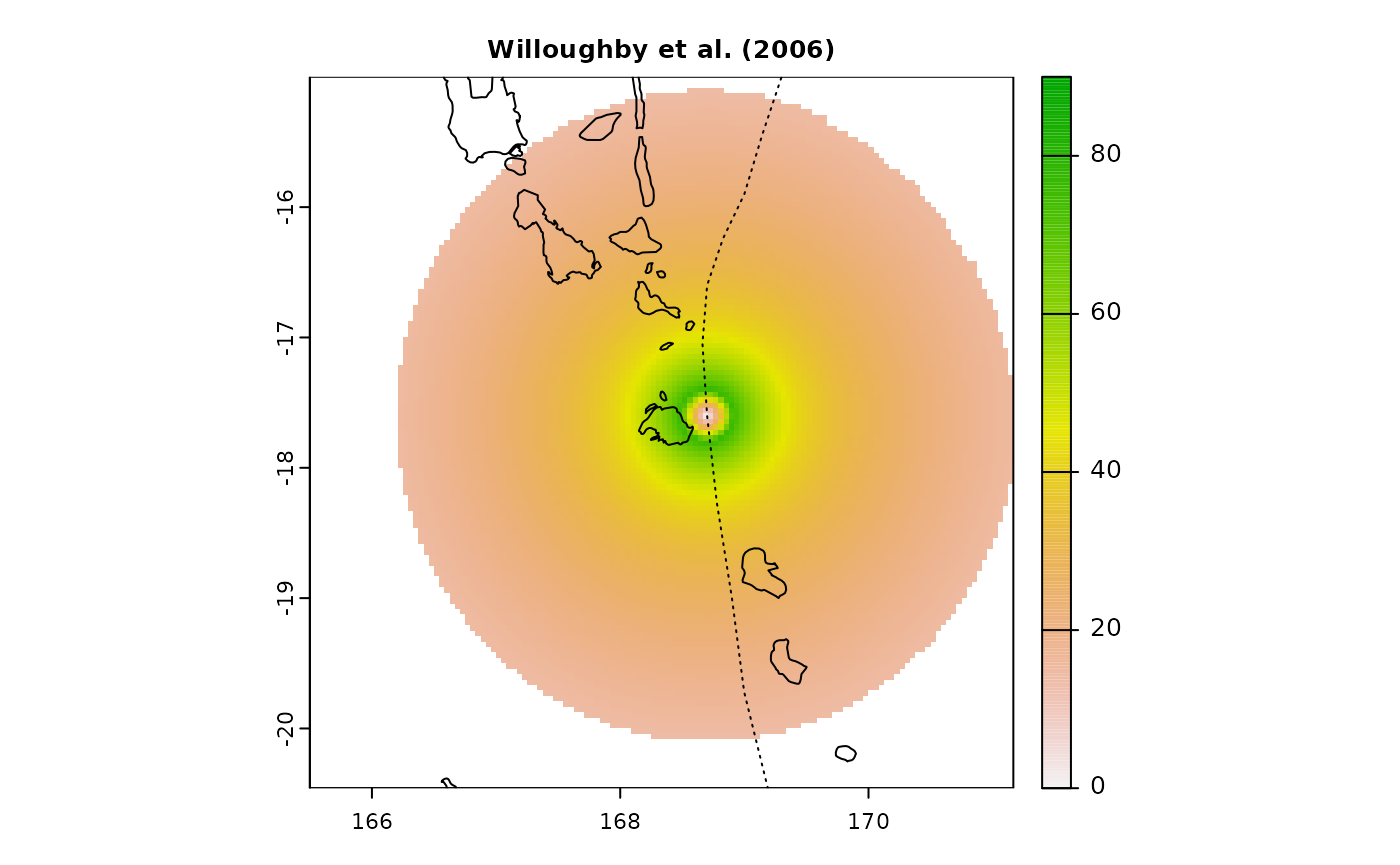
\includegraphics{Models_files/figure-latex/unnamed-chunk-2-2.pdf}

\begin{Shaded}
\begin{Highlighting}[]
\FunctionTok{par}\NormalTok{(}\AttributeTok{mfrow=}\FunctionTok{c}\NormalTok{(}\DecValTok{1}\NormalTok{,}\DecValTok{2}\NormalTok{))}
\NormalTok{pf }\OtherTok{\textless{}{-}} \FunctionTok{spatialBehaviour}\NormalTok{(st,}\AttributeTok{product=}\StringTok{"Profiles"}\NormalTok{,}\AttributeTok{method=}\StringTok{"Holland"}\NormalTok{,}\AttributeTok{asymmetry=}\StringTok{"Chen"}\NormalTok{,}\AttributeTok{verbose=}\DecValTok{0}\NormalTok{)}
\NormalTok{terra}\SpecialCharTok{::}\FunctionTok{plot}\NormalTok{(pf}\SpecialCharTok{$}\NormalTok{PAM\_Speed\_41,}\AttributeTok{main=}\StringTok{"Holland (1980) + Chen (1994)"}\NormalTok{,}\AttributeTok{cex.main=}\FloatTok{0.8}\NormalTok{)}
\NormalTok{terra}\SpecialCharTok{::}\FunctionTok{plot}\NormalTok{(countriesHigh,}\AttributeTok{add=}\ConstantTok{TRUE}\NormalTok{)}
\FunctionTok{lines}\NormalTok{(PAM}\SpecialCharTok{$}\NormalTok{lon,PAM}\SpecialCharTok{$}\NormalTok{lat,}\AttributeTok{lty=}\DecValTok{3}\NormalTok{)}
\NormalTok{pf }\OtherTok{\textless{}{-}} \FunctionTok{spatialBehaviour}\NormalTok{(st,}\AttributeTok{product=}\StringTok{"Profiles"}\NormalTok{,}\AttributeTok{method=}\StringTok{"Willoughby"}\NormalTok{,}\AttributeTok{asymmetry=}\StringTok{"Chen"}\NormalTok{,}\AttributeTok{verbose=}\DecValTok{0}\NormalTok{)}
\NormalTok{terra}\SpecialCharTok{::}\FunctionTok{plot}\NormalTok{(pf}\SpecialCharTok{$}\NormalTok{PAM\_Speed\_41,}\AttributeTok{main=}\StringTok{"Willoughby et al. (2006) + Chen (1994)"}\NormalTok{,}\AttributeTok{cex.main=}\FloatTok{0.8}\NormalTok{)}
\NormalTok{terra}\SpecialCharTok{::}\FunctionTok{plot}\NormalTok{(countriesHigh,}\AttributeTok{add=}\ConstantTok{TRUE}\NormalTok{)}
\FunctionTok{lines}\NormalTok{(PAM}\SpecialCharTok{$}\NormalTok{lon,PAM}\SpecialCharTok{$}\NormalTok{lat,}\AttributeTok{lty=}\DecValTok{3}\NormalTok{)}
\end{Highlighting}
\end{Shaded}

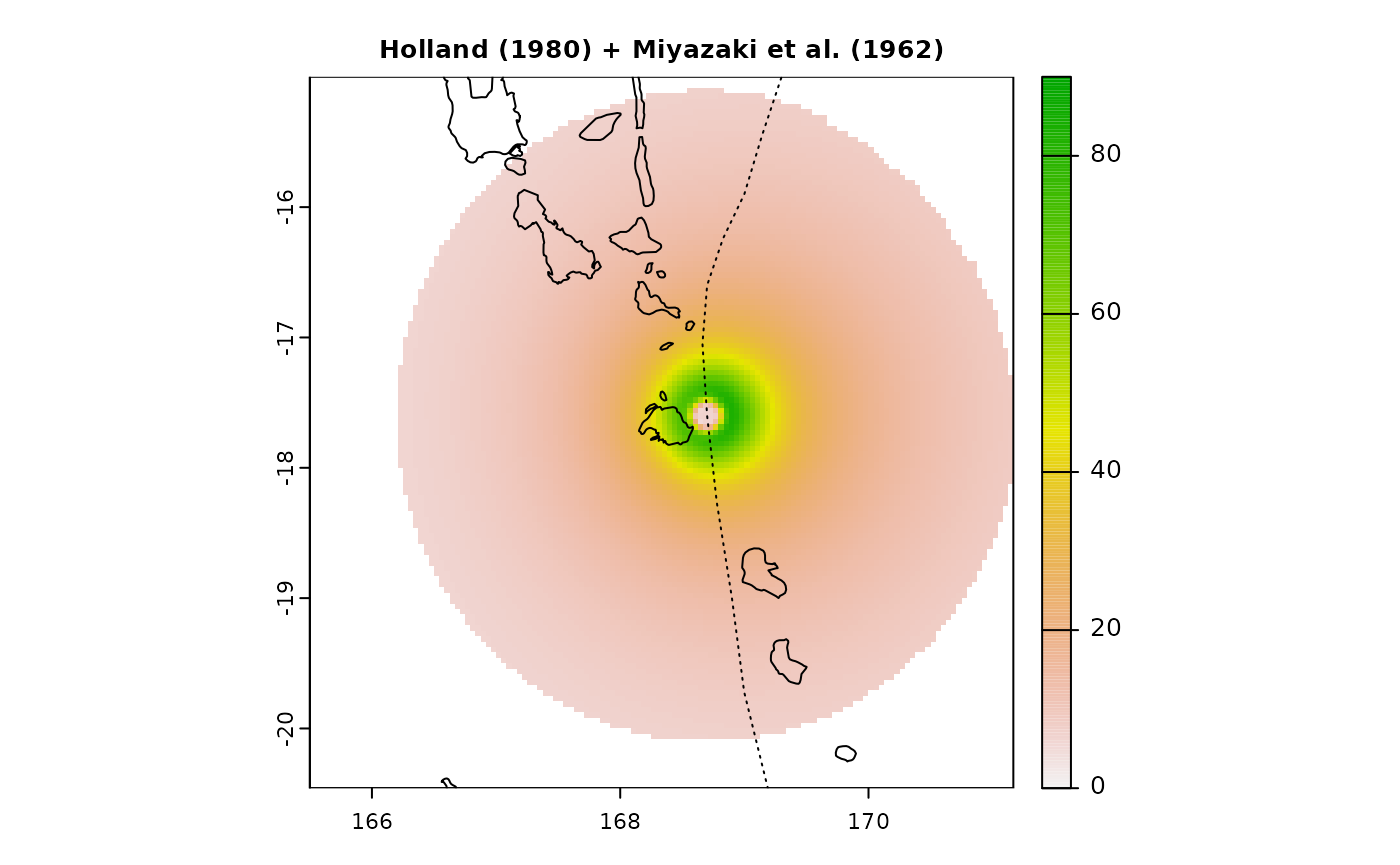
\includegraphics{Models_files/figure-latex/unnamed-chunk-2-3.pdf}

\begin{Shaded}
\begin{Highlighting}[]
\FunctionTok{par}\NormalTok{(}\AttributeTok{mfrow=}\FunctionTok{c}\NormalTok{(}\DecValTok{1}\NormalTok{,}\DecValTok{2}\NormalTok{))}
\NormalTok{pf }\OtherTok{\textless{}{-}} \FunctionTok{spatialBehaviour}\NormalTok{(st,}\AttributeTok{product=}\StringTok{"Profiles"}\NormalTok{,}\AttributeTok{method=}\StringTok{"Boose"}\NormalTok{,}\AttributeTok{verbose=}\DecValTok{0}\NormalTok{)}
\NormalTok{terra}\SpecialCharTok{::}\FunctionTok{plot}\NormalTok{(pf}\SpecialCharTok{$}\NormalTok{PAM\_Speed\_41,}\AttributeTok{main=}\StringTok{"Boose et al. (2004)"}\NormalTok{,}\AttributeTok{cex.main=}\FloatTok{0.8}\NormalTok{)}
\NormalTok{terra}\SpecialCharTok{::}\FunctionTok{plot}\NormalTok{(countriesHigh,}\AttributeTok{add=}\ConstantTok{TRUE}\NormalTok{)}
\FunctionTok{lines}\NormalTok{(PAM}\SpecialCharTok{$}\NormalTok{lon,PAM}\SpecialCharTok{$}\NormalTok{lat,}\AttributeTok{lty=}\DecValTok{3}\NormalTok{)}
\end{Highlighting}
\end{Shaded}

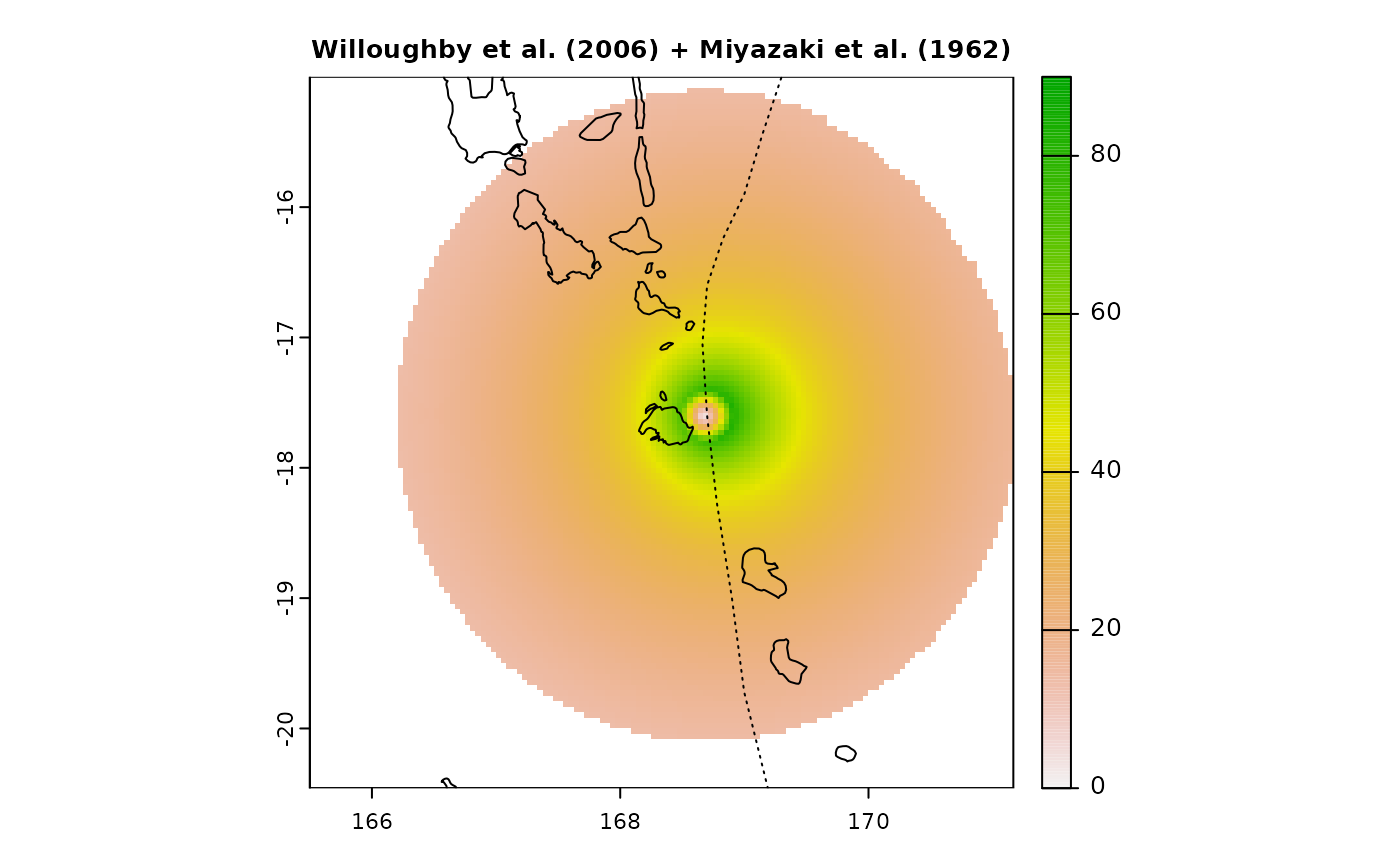
\includegraphics{Models_files/figure-latex/unnamed-chunk-2-4.pdf}

\hypertarget{wind-direction}{%
\subsubsection{Wind direction}\label{wind-direction}}

Regardless of the model used of wind speed, wind direction is computed
as follows:

\[
\left\{
\begin{aligned}
D = A_z - 90 - I \quad if \quad \phi > 0 \quad(Northern \quad Hemispher) \\
D = A_z - 90 - I \quad if \quad \phi \leq 0 \quad(Southern \quad Hemispher) \\
\end{aligned}
\right.
\] where \(D\) is the direction of the radial wind \(A_z\) is the
azimuth from point r to the eye of the storm \(I\) is the cross isobar
inflow angle (\(20\) in water, \(40\) in land) \(\phi\) is the latitude

\hypertarget{references}{%
\subsection{References}\label{references}}

\begin{itemize}
\item
  Boose, E. R., Chamberlin, K. E., \& Foster, D. R. (2001). Landscape
  and Regional Impacts of Hurricanes in New England. Ecological
  Monographs, 71(1), Article 1.
  \url{https://doi.org/10.1890/0012-9615(2001)071\%5B0027:LARIOH\%5D2.0.CO;2}
\item
  Boose, E. R., Serrano, M. I., \& Foster, D. R. (2004). Landscape and
  regional impacts of hurricanes in Puerto Rico. Ecological Monographs,
  74(2), Article 2. \url{https://doi.org/10.1890/02-4057}
\item
  Holland, G. J. (1980). An Analytic Model of the Wind and Pressure
  Profiles in Hurricanes. Monthly Weather Review, 108(8), 1212--1218.
  \url{https://doi.org/10.1175/1520-0493(1980)108}\textless1212:AAMOTW\textgreater2.0.CO;2
\item
  Willoughby, H. E. (1995). Normal-Mode Initialization of Barotropic
  Vortex Motion Models. Journal of the Atmospheric Sciences, 52(24),
  4501--4514.
  \url{https://doi.org/10.1175/1520-0469(1995)052}\textless4501:NMIOBV\textgreater2.0.CO;2
\item
  Willoughby, H. E., \& Rahn, M. E. (2004). Parametric Representation of
  the Primary Hurricane Vortex. Part I: Observations and Evaluation of
  the Holland (1980) Model. Monthly Weather Review, 132(12), 3033--3048.
  \url{https://doi.org/10.1175/MWR2831.1}
\item
  Willoughby, H. E., Darling, R. W. R., \& Rahn, M. E. (2006).
  Parametric Representation of the Primary Hurricane Vortex. Part II: A
  New Family of Sectionally Continuous Profiles. Monthly Weather Review,
  134(4), 1102--1120. \url{https://doi.org/10.1175/MWR3106.1}
\item
  Yan, D., \& Zhang, T. (2022). Research progress on tropical cyclone
  parametric wind field models and their application. Regional Studies
  in Marine Science, 51, 102207.
  \url{https://doi.org/10.1016/j.rsma.2022.102207}
\end{itemize}

\end{document}
